% Options for packages loaded elsewhere
\PassOptionsToPackage{unicode}{hyperref}
\PassOptionsToPackage{hyphens}{url}
%
\documentclass[
]{book}
\usepackage{lmodern}
\usepackage{amssymb,amsmath}
\usepackage{ifxetex,ifluatex}
\ifnum 0\ifxetex 1\fi\ifluatex 1\fi=0 % if pdftex
  \usepackage[T1]{fontenc}
  \usepackage[utf8]{inputenc}
  \usepackage{textcomp} % provide euro and other symbols
\else % if luatex or xetex
  \usepackage{unicode-math}
  \defaultfontfeatures{Scale=MatchLowercase}
  \defaultfontfeatures[\rmfamily]{Ligatures=TeX,Scale=1}
\fi
% Use upquote if available, for straight quotes in verbatim environments
\IfFileExists{upquote.sty}{\usepackage{upquote}}{}
\IfFileExists{microtype.sty}{% use microtype if available
  \usepackage[]{microtype}
  \UseMicrotypeSet[protrusion]{basicmath} % disable protrusion for tt fonts
}{}
\makeatletter
\@ifundefined{KOMAClassName}{% if non-KOMA class
  \IfFileExists{parskip.sty}{%
    \usepackage{parskip}
  }{% else
    \setlength{\parindent}{0pt}
    \setlength{\parskip}{6pt plus 2pt minus 1pt}}
}{% if KOMA class
  \KOMAoptions{parskip=half}}
\makeatother
\usepackage{xcolor}
\IfFileExists{xurl.sty}{\usepackage{xurl}}{} % add URL line breaks if available
\IfFileExists{bookmark.sty}{\usepackage{bookmark}}{\usepackage{hyperref}}
\hypersetup{
  pdftitle={Estimating Social Animal Models in Stan},
  pdfauthor={Jordan S. Martin \& Adrian V. Jaeggi},
  hidelinks,
  pdfcreator={LaTeX via pandoc}}
\urlstyle{same} % disable monospaced font for URLs
\usepackage{color}
\usepackage{fancyvrb}
\newcommand{\VerbBar}{|}
\newcommand{\VERB}{\Verb[commandchars=\\\{\}]}
\DefineVerbatimEnvironment{Highlighting}{Verbatim}{commandchars=\\\{\}}
% Add ',fontsize=\small' for more characters per line
\usepackage{framed}
\definecolor{shadecolor}{RGB}{248,248,248}
\newenvironment{Shaded}{\begin{snugshade}}{\end{snugshade}}
\newcommand{\AlertTok}[1]{\textcolor[rgb]{0.94,0.16,0.16}{#1}}
\newcommand{\AnnotationTok}[1]{\textcolor[rgb]{0.56,0.35,0.01}{\textbf{\textit{#1}}}}
\newcommand{\AttributeTok}[1]{\textcolor[rgb]{0.77,0.63,0.00}{#1}}
\newcommand{\BaseNTok}[1]{\textcolor[rgb]{0.00,0.00,0.81}{#1}}
\newcommand{\BuiltInTok}[1]{#1}
\newcommand{\CharTok}[1]{\textcolor[rgb]{0.31,0.60,0.02}{#1}}
\newcommand{\CommentTok}[1]{\textcolor[rgb]{0.56,0.35,0.01}{\textit{#1}}}
\newcommand{\CommentVarTok}[1]{\textcolor[rgb]{0.56,0.35,0.01}{\textbf{\textit{#1}}}}
\newcommand{\ConstantTok}[1]{\textcolor[rgb]{0.00,0.00,0.00}{#1}}
\newcommand{\ControlFlowTok}[1]{\textcolor[rgb]{0.13,0.29,0.53}{\textbf{#1}}}
\newcommand{\DataTypeTok}[1]{\textcolor[rgb]{0.13,0.29,0.53}{#1}}
\newcommand{\DecValTok}[1]{\textcolor[rgb]{0.00,0.00,0.81}{#1}}
\newcommand{\DocumentationTok}[1]{\textcolor[rgb]{0.56,0.35,0.01}{\textbf{\textit{#1}}}}
\newcommand{\ErrorTok}[1]{\textcolor[rgb]{0.64,0.00,0.00}{\textbf{#1}}}
\newcommand{\ExtensionTok}[1]{#1}
\newcommand{\FloatTok}[1]{\textcolor[rgb]{0.00,0.00,0.81}{#1}}
\newcommand{\FunctionTok}[1]{\textcolor[rgb]{0.00,0.00,0.00}{#1}}
\newcommand{\ImportTok}[1]{#1}
\newcommand{\InformationTok}[1]{\textcolor[rgb]{0.56,0.35,0.01}{\textbf{\textit{#1}}}}
\newcommand{\KeywordTok}[1]{\textcolor[rgb]{0.13,0.29,0.53}{\textbf{#1}}}
\newcommand{\NormalTok}[1]{#1}
\newcommand{\OperatorTok}[1]{\textcolor[rgb]{0.81,0.36,0.00}{\textbf{#1}}}
\newcommand{\OtherTok}[1]{\textcolor[rgb]{0.56,0.35,0.01}{#1}}
\newcommand{\PreprocessorTok}[1]{\textcolor[rgb]{0.56,0.35,0.01}{\textit{#1}}}
\newcommand{\RegionMarkerTok}[1]{#1}
\newcommand{\SpecialCharTok}[1]{\textcolor[rgb]{0.00,0.00,0.00}{#1}}
\newcommand{\SpecialStringTok}[1]{\textcolor[rgb]{0.31,0.60,0.02}{#1}}
\newcommand{\StringTok}[1]{\textcolor[rgb]{0.31,0.60,0.02}{#1}}
\newcommand{\VariableTok}[1]{\textcolor[rgb]{0.00,0.00,0.00}{#1}}
\newcommand{\VerbatimStringTok}[1]{\textcolor[rgb]{0.31,0.60,0.02}{#1}}
\newcommand{\WarningTok}[1]{\textcolor[rgb]{0.56,0.35,0.01}{\textbf{\textit{#1}}}}
\usepackage{longtable,booktabs}
% Correct order of tables after \paragraph or \subparagraph
\usepackage{etoolbox}
\makeatletter
\patchcmd\longtable{\par}{\if@noskipsec\mbox{}\fi\par}{}{}
\makeatother
% Allow footnotes in longtable head/foot
\IfFileExists{footnotehyper.sty}{\usepackage{footnotehyper}}{\usepackage{footnote}}
\makesavenoteenv{longtable}
\usepackage{graphicx,grffile}
\makeatletter
\def\maxwidth{\ifdim\Gin@nat@width>\linewidth\linewidth\else\Gin@nat@width\fi}
\def\maxheight{\ifdim\Gin@nat@height>\textheight\textheight\else\Gin@nat@height\fi}
\makeatother
% Scale images if necessary, so that they will not overflow the page
% margins by default, and it is still possible to overwrite the defaults
% using explicit options in \includegraphics[width, height, ...]{}
\setkeys{Gin}{width=\maxwidth,height=\maxheight,keepaspectratio}
% Set default figure placement to htbp
\makeatletter
\def\fps@figure{htbp}
\makeatother
\setlength{\emergencystretch}{3em} % prevent overfull lines
\providecommand{\tightlist}{%
  \setlength{\itemsep}{0pt}\setlength{\parskip}{0pt}}
\setcounter{secnumdepth}{5}
\usepackage{booktabs}
\usepackage[]{natbib}
\bibliographystyle{apalike}

\title{Estimating Social Animal Models in Stan}
\author{Jordan S. Martin \& Adrian V. Jaeggi}
\date{2021-01-06}

\begin{document}
\maketitle

{
\setcounter{tocdepth}{1}
\tableofcontents
}
\hypertarget{introduction}{%
\chapter*{Introduction}\label{introduction}}
\addcontentsline{toc}{chapter}{Introduction}

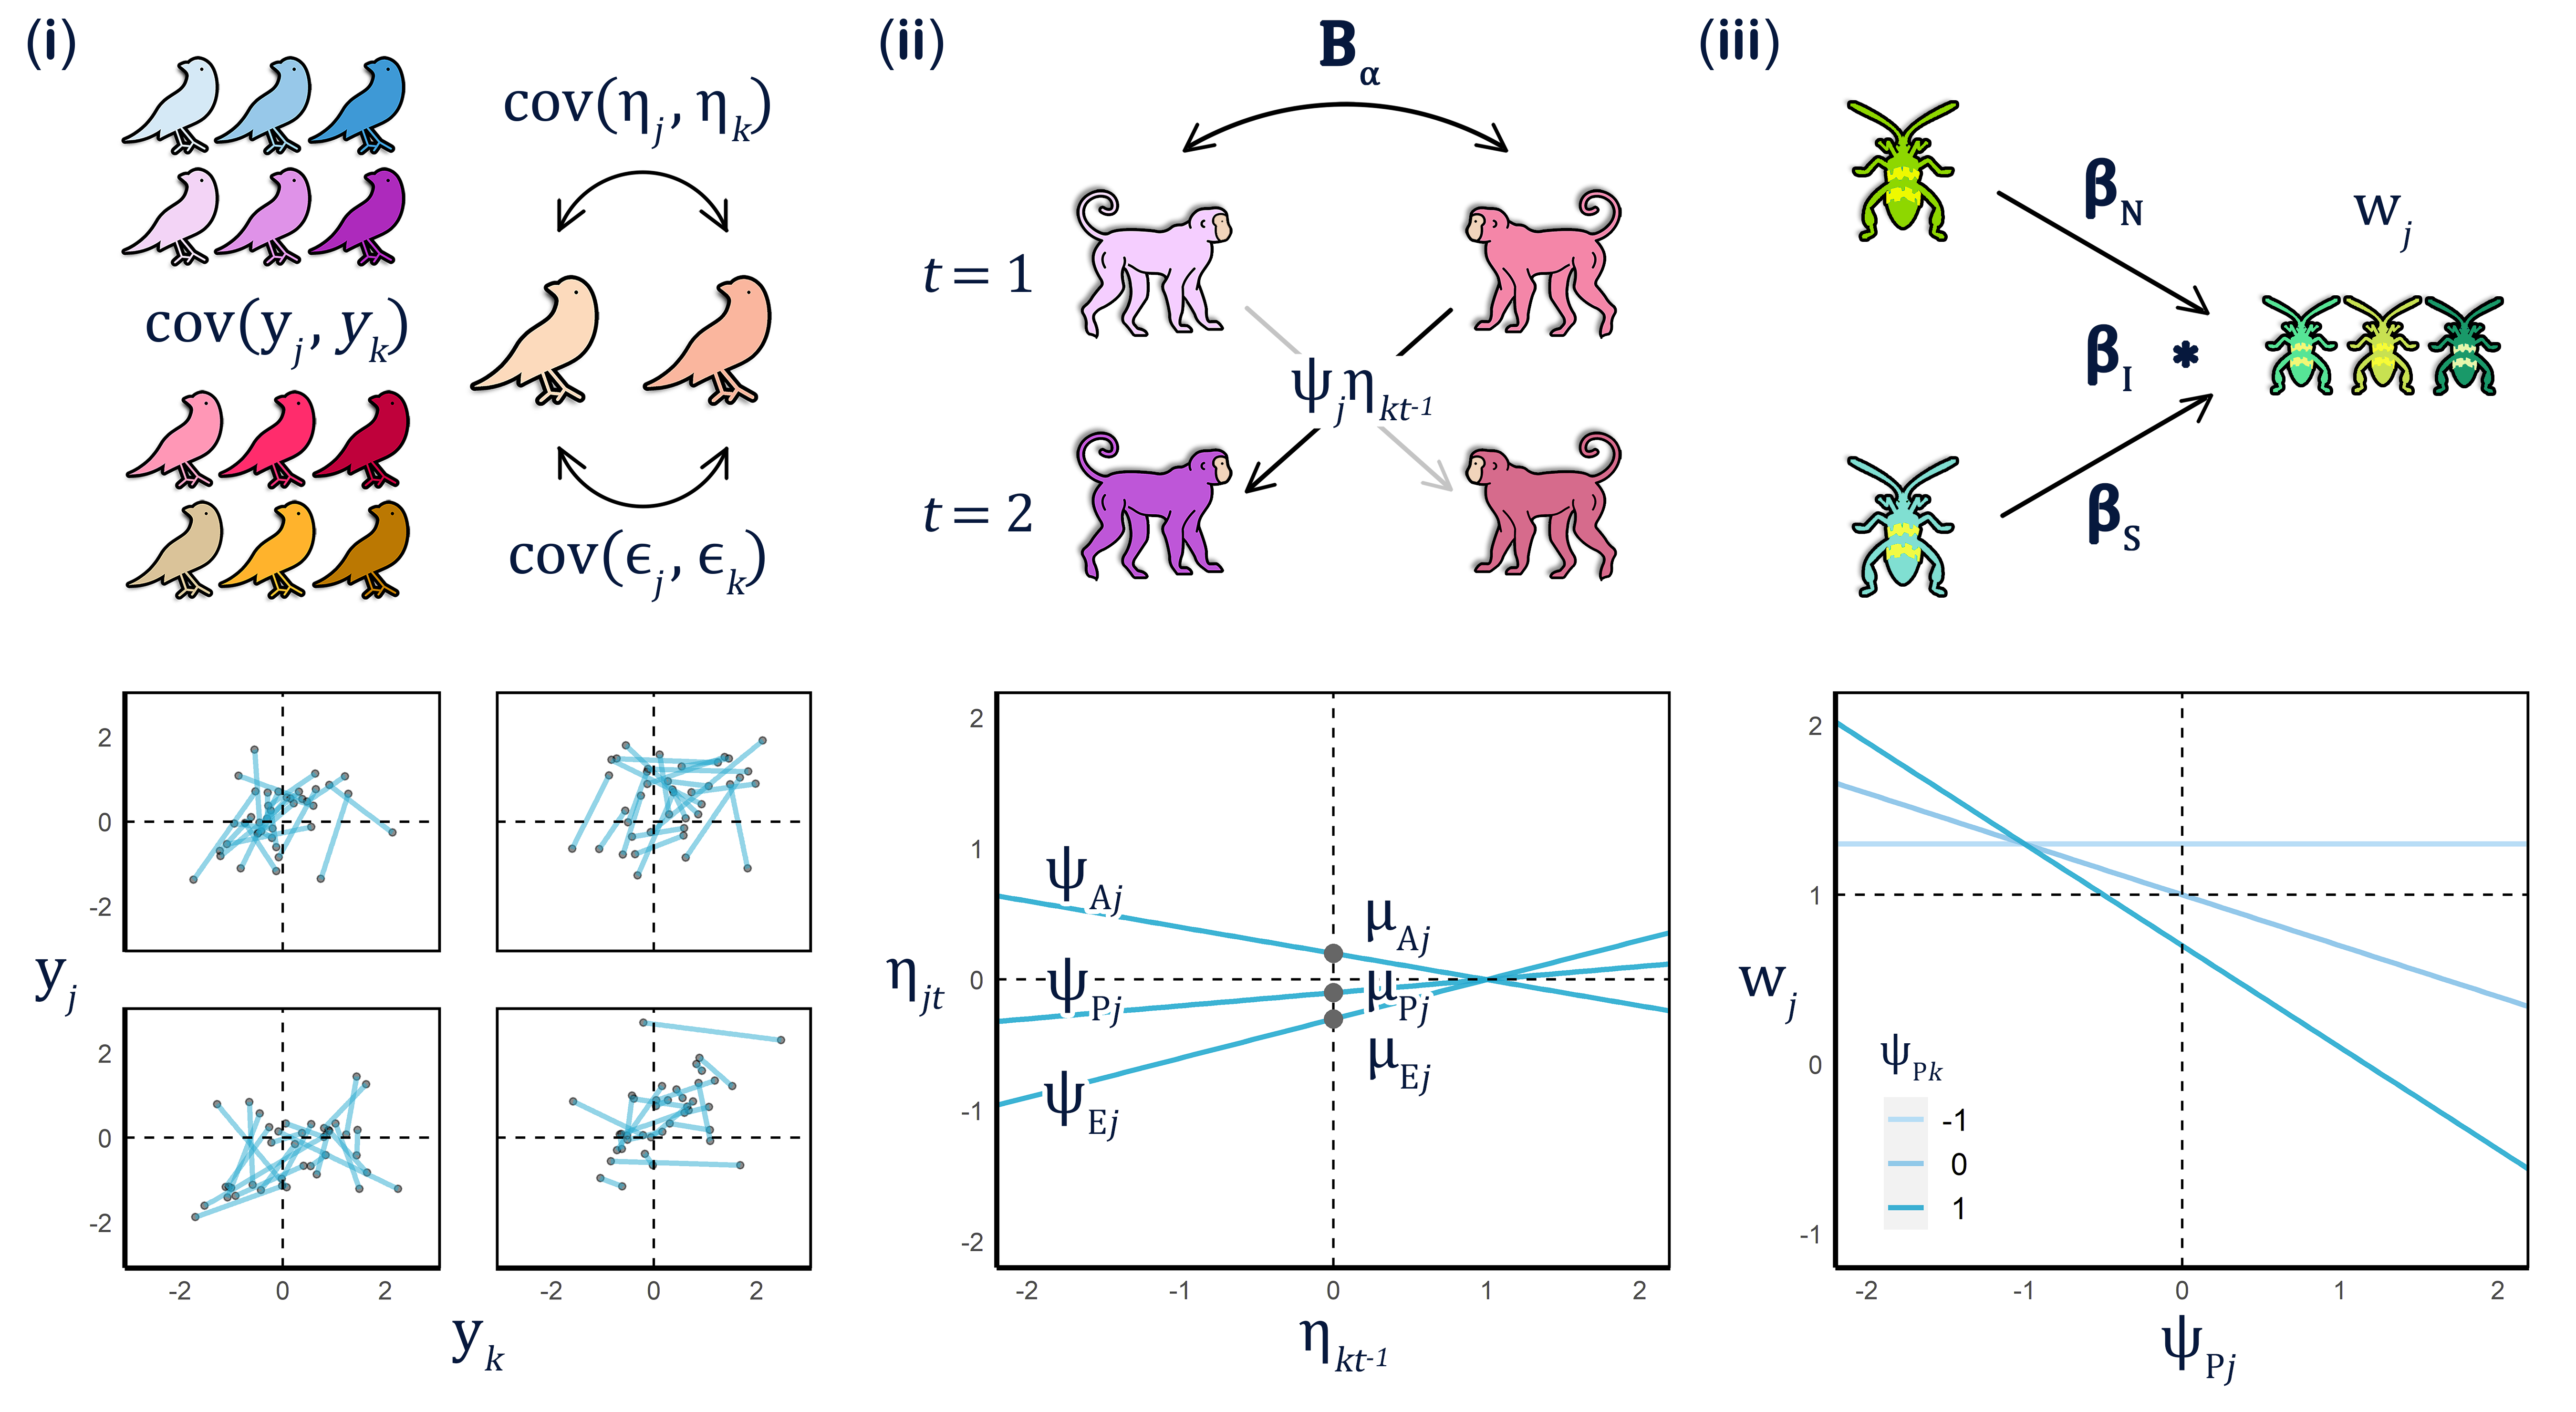
\includegraphics{Fig 1 r1.png}

This guidebook provides a comprehensive overview of how to estimate social animal models (SAMs) with the Stan statistical programming language \citep{Stan} in R \citep{Rbase}. A detailed theoretical treatment of SAMs and their empirical motivation can be found in the forthcoming paper \citep{SAM} ``Social animal models for quantifying plasticity, assortment, and selection on interacting phenotypes'' in the \emph{Journal of Evolutionary Biology}. This guide focuses on additional issues related to coding SAMs in Stan, as well as the extension of SAMs beyond the Gaussian response models presented in the main text. The overarching goal of the guidebook is to aid researchers in flexibly and appropriately applying SAMs to their own empirical datasets. Therefore, in addition to basic coding tutorials, the guide also includes a growing body of worked examples relevant to specific challenges such as modeling spatial autocorrelation or hierarchical phenotypes.

Please contact \href{mailto:jordan.martin@iem.uzh.ch?}{Jordan Scott Martin} to suggest any additional examples of interest to your own work. The guidebook is a work in progress and will be continuously updated over time.

\hypertarget{using-stan-in-r}{%
\chapter{Using Stan in R}\label{using-stan-in-r}}

\hypertarget{why-stan}{%
\section{Why Stan?}\label{why-stan}}

SAMs cannot be straightforwardly implemented with currently available software for quantitative genetic analysis, such as the frequentist ASREML program \citep{ASREML} or the Bayesian open-source R package MCMCglmm \citep{MCMCglmm}. The classical animal models estimated by these programs can be used to describe reaction norms defined over non-social environments, with reaction norm slopes estimated on directly measured environmental gradients. However, social environments defined by partner phenotypes present novel challenges for animal models, such as accounting for temporal feedback between social partners' phenotypes, differentiating the effects of assortment and social plasticity between partners, and avoiding bias due to correlated residual effects on measurements taken within and among social interactions \citep{SAM}. SAMs address these challenges by estimating plasticity, assortment, and selection directly on the latent social reaction norms (SRNs) governing repeatable individual variation. A highly flexible modeling framework is required to estimate these latent (i.e.~indirectly measured) interactions with raw empirical data, as well as to use them for predicting social evolutionary change.

Stan \citep{Stan} is an open-source programming language for estimating probabilistic models of arbitrary complexity, which can interface with multiple statistical environments such as R \citep{Rbase}. Stan also facilitates fully Bayesian inference using state-of-the-art Markov Chain Monte Carlo (MCMC) sampling techniques. In particular, the No U-Turn Sampler (NUTS) implimented in Stan has been found to perform particularly well for quantitative genetic analysis \citep{MCMCperf}. Stan is thus an ideal platform for flexibly estimating SAMs in any empirical system, as is further discussed in the main text \citep{SAM}. Using Bayesian posteriors rather than point estimates will also promote more robust biological inferences with SAMs, as statistical uncertainty can be easily carried forward across multiple stages of analysis \citep{Stinchcombe2014}. This provides a crucial means of quantifying uncertainty in the predicted direction and magnitude of social evolution.

\hypertarget{getting-started}{%
\section{Getting Started}\label{getting-started}}

Stan interfaces with R through the RStan package \citep{Stan}, providing an efficient means of integrating SAMs into pre-existing data analysis pipelines. However, you will first need to install Stan on your computer and ensure that it is appropriately configured with your C++ toolchain. This can be accomplished by following the instructions for your operating system on the \href{https://github.com/stan-dev/rstan/wiki/RStan-Getting-Started}{RStan Getting Started} page. Once you are able to effectively use RStan, you can begin creating the \texttt{.stan} files necessary for estimating SAMs. These files can be composed using RStudio or any text editor, as explained below. Once an appropriate \texttt{.stan} file is prepared, it can be compiled with R for the C++ toolchain using the \texttt{stan\_model()} function and subsequently estimated with an appropriate list of empirical data using the \texttt{sampling()} function. The resulting posteriors of a model can then be accessed with the \texttt{extract()} function and manipulated for any further quantities or analyses of interest.

\begin{Shaded}
\begin{Highlighting}[]
\KeywordTok{library}\NormalTok{(rstan)}

\CommentTok{#compiles the model in C++ for MCMC estimation}
\NormalTok{model =}\StringTok{ }\KeywordTok{stan_model}\NormalTok{(}\StringTok{"model.stan"}\NormalTok{)}

\CommentTok{#estimates and saves the posterior MCMC samples of the model (estimated with default settings)}
\NormalTok{results =}\StringTok{ }\KeywordTok{sampling}\NormalTok{(}\DataTypeTok{object =}\NormalTok{ SAM_file, }\DataTypeTok{data =}\NormalTok{ data)}

\CommentTok{#extracts posterior estimates}
\NormalTok{MCMCsamples =}\StringTok{  }\KeywordTok{extract}\NormalTok{(results)}
\end{Highlighting}
\end{Shaded}

\hypertarget{bayesian-inference}{%
\section{Bayesian inference}\label{bayesian-inference}}

A detailed overview of the benefits of Bayesian inference is beyond the scope of this guidebook, as attention is placed on coding and computational concerns rather than interpretation. We encourage researchers unfamiliar with fully Bayesian inference to see \citet{Rethinking} for further discussion. \citet{Lemoine2019} also demonstrates why weakly regularizing (or ``weakly informative'') priors are often preferable to the flat or diffuse priors more commonly used in evolutionary ecology. In general, we encourage researchers to utilize the benefits of fully Bayesian inference while working in Stan, rather than attempting to mimic classical inference and null-hypothesis testing approaches. \citet{Gelman2020} provide a very useful general discussion of Bayesian workflow from initial estimation to model comparison and selection. A basic understanding of MCMC and prior and posterior distributions is necessary to fully understand model estimation in Stan. MCMC provides a means of approximating any continous probability distribution, with a finite set of samples taken in proportion to the underlying target probability density. As a consequence, Stan models return objects with many MCMC samples for each model parameter, rather than single point estimates. These samples can then be summarized to approximate the shape of the truly continous target posterior distribution, as is shown throughout the coding tutorials.

\hypertarget{basic-coding-tutorial}{%
\section{Basic coding tutorial}\label{basic-coding-tutorial}}

Stan uses its own language for writing probabilistic models, including a variety of built-in functions designed to aid in efficient computation. The biggest conceptual hurdle for new users of Stan is likely to be the absence of an intuitive R-like syntax for specifying model formulas, such as formulas like \texttt{y\ \textasciitilde{}\ x\ +\ (1\textbar{}z)} that can be used to quickly specify complex generalized linear mixed-effects models. These formulas facilitate highly efficient statistical modeling, but do so at the cost of limiting users' ability to specify atypical model structures. Instead, Stan provides the benefit of nearly unlimited flexibility in model specification, with the added cost of a steeper learning curve. In particular, models must be formally specified with mathematically appropriate likelihood functions, rather than this process being handled on the back-end through textual inputs from the user such as \texttt{family=\ poisson(link\ =\ "log")}. This may at first seem like a cumbersome task, but it provides a degree of independence and creativity for data analysis that is otherwise unavailable. It is this autonomy that makes it possible to unbiasedly estimate SAMs in Stan, which to the best of our knowledge cannot be accomplished with any other mainstream statistical software. Nonetheless, it is important to recognize that some practice and trial-and-error will be required to gain competency and comfortability with Stan. We therefore encourage those interested in SAMs to review the \href{https://mc-stan.org/docs/2_25/reference-manual/index.html}{Stan Reference Manual}, as well the extensive collection of \href{https://mc-stan.org/users/documentation/case-studies}{Stan Case Studies}, which will provide a more robust foundation for estimating any model of interest in Stan.

Here we review some basics of Stan that will be necessary for following the coding tutorials in the rest of the guidebook. To make this introduction more concrete, we simulate a simple data structure appropriately described by a Gaussian random regression model, with 50 subjects and 2 repeated measures per subject across an environmental gradient \(x\). Formally, the model for observation \emph{i} of individual \emph{j} is given by

\[y_{ij}=\mu_{j}+\beta_{j}x_{ij}+\epsilon_i\]
\[\mu_j=\mu_0+\mu_{\mathrm{P}j},  \quad  \beta_j=\beta_1+\beta_{\mathrm{P}j}\]

\[ \begin{bmatrix}
\boldsymbol{\mu_{\mathrm{P}}} \\ 
\boldsymbol{\beta_{\mathrm{P}}} 
\end{bmatrix} \sim \mathrm{MVNormal}(\boldsymbol{0}, \boldsymbol{\mathrm{P}} ) : 
\boldsymbol{\mathrm{P}} =
\begin{bmatrix}
\mathrm{Var}( \boldsymbol{\mu_{\mathrm{P}}} ) &  
\mathrm{Cov}( \boldsymbol{\mu_{\mathrm{P}}},  \boldsymbol{\beta_{\mathrm{P}}})     \\ 
\mathrm{Cov}(\boldsymbol{\beta_{\mathrm{P}}}, \boldsymbol{\mu_{\mathrm{P}}} ) & 
\mathrm{Var}( \boldsymbol{\beta_{\mathrm{P}}} )
\end{bmatrix} \]

\[ \boldsymbol{\epsilon} \sim \mathrm{Normal}(0, \boldsymbol{\mathrm{R}} ): 
\boldsymbol{\mathrm{R}} =
[\mathrm{Var}(\boldsymbol{\epsilon})]\]

where \(\mu_0\) and \(\beta_1\) are fixed population-level intercepts and slopes respectively, with the vectors \(\boldsymbol{\mu_{\mathrm{P}}}\) and \(\boldsymbol{\beta_{\mathrm{P}}}\) containing individual-specific phenotypic deviations from the population values (i.e.~random intercepts and slopes). The probability density function of this Gaussian variable can be equivalently written as

\[y_{ij} \sim \mathrm{Normal}(\mu_{j}+\beta_{j}x_{ij},\mathrm{Var}(\boldsymbol{\epsilon}))\]
It is often easier to specify model likelihoods and priors over standard deviations and correlation matrices in Stan, rather than the variances and covariances represented in the formal model. These parameters can always be derived from one another with simple transformations. For variances and standard deviations

\[\mathrm{SD}( \boldsymbol{\mu_{\mathrm{P}}}  ) = \mathrm{Sqrt(Var} (\boldsymbol{\boldsymbol{\mu_{\mathrm{P}}} }) ) , \quad \mathrm{SD}( \boldsymbol{\beta_{\mathrm{P}}}  ) = \mathrm{Sqrt(Var} (\boldsymbol{\boldsymbol{\beta_{\mathrm{P}}} }) )\]

Similarly, the covariance matrix \(\boldsymbol{\mathrm{P}}\) can be derived by pre- and post-multiplying the correlation matrix \(\boldsymbol{\mathrm{P_{Cor}}}\) with diagonal matrices \(\boldsymbol{\mathrm{P_{SD}}}\) of these standard deviations

\[\boldsymbol{\mathrm{P}} =  \boldsymbol{\mathrm{P_{SD}}} \boldsymbol{\mathrm{P_{Cor}}} \boldsymbol{\mathrm{P_{SD}}}\]

\[ \boldsymbol{\mathrm{P_{SD}}} = \begin{bmatrix} \mathrm{SD}( \boldsymbol{\mu_{\mathrm{P}}} )     &  0    \\ 
0     &     \mathrm{SD}( \boldsymbol{\beta_{\mathrm{P}}} ) \end{bmatrix}, \quad 
 \boldsymbol{\mathrm{P_{Cor}}} = \begin{bmatrix} 1     &  \mathrm{Cor}( \boldsymbol{\mu_{\mathrm{P}}}, \boldsymbol{\beta_{\mathrm{P}}} )    \\ 
\mathrm{Cor}( \boldsymbol{\beta_{\mathrm{P}}} , \boldsymbol{\mu_{\mathrm{P}}} )      &    1
\end{bmatrix} \]

We can simulate a random dataset from this model in R, along with an index variable \texttt{id} that tracks which individual (I = 1 - 50) is being measured at each observation (N = 1-100).

\begin{Shaded}
\begin{Highlighting}[]
\KeywordTok{library}\NormalTok{(mvtnorm)}

\NormalTok{N =}\StringTok{ }\DecValTok{100} \CommentTok{#total observations}
\NormalTok{I =}\StringTok{ }\DecValTok{50} \CommentTok{#total individuals}

\NormalTok{intercept =}\StringTok{ }\DecValTok{1} \CommentTok{#global intercept}
\NormalTok{beta1 =}\StringTok{ }\FloatTok{0.3} \CommentTok{#fixed effect regression coefficient}
\NormalTok{SD_intercept =}\StringTok{ }\FloatTok{0.3} \CommentTok{#standard deviation of random intercepts}
\NormalTok{SD_slope =}\StringTok{ }\FloatTok{0.3}
\NormalTok{SD_residual =}\StringTok{ }\DecValTok{1}
\NormalTok{cor_RE =}\StringTok{ }\FloatTok{0.3} \CommentTok{#correlation of random intercepts and slopes}

\CommentTok{#individual-level index}
\NormalTok{id =}\StringTok{ }\KeywordTok{rep}\NormalTok{(}\KeywordTok{seq}\NormalTok{(}\DecValTok{1}\NormalTok{, I), }\DataTypeTok{each =}\NormalTok{ N}\OperatorTok{/}\NormalTok{I) }\CommentTok{#i.e. two observations per individual}

\CommentTok{#simulate fixed effect covariate}
\NormalTok{x =}\StringTok{ }\KeywordTok{rnorm}\NormalTok{(}\DecValTok{100}\NormalTok{,}\DecValTok{0}\NormalTok{,}\DecValTok{1}\NormalTok{) }\CommentTok{#fixed effect covariate}

\CommentTok{#simulate random individual deviations}
\NormalTok{P_cor =}\StringTok{ }\KeywordTok{matrix}\NormalTok{( }\KeywordTok{c}\NormalTok{(}\DecValTok{1}\NormalTok{, cor_RE, cor_RE, }\DecValTok{1}\NormalTok{), }\DataTypeTok{nrow =} \DecValTok{2}\NormalTok{, }\DataTypeTok{ncol =} \DecValTok{2}\NormalTok{ )}
\NormalTok{P_SD =}\StringTok{ }\KeywordTok{matrix}\NormalTok{( }\KeywordTok{c}\NormalTok{(SD_intercept, }\DecValTok{0}\NormalTok{, }\DecValTok{0}\NormalTok{, SD_slope), }\DataTypeTok{nrow =} \DecValTok{2}\NormalTok{, }\DataTypeTok{ncol =} \DecValTok{2}\NormalTok{ )}
\NormalTok{P_cov =}\StringTok{ }\NormalTok{P_SD }\OperatorTok\StringTok{ }\NormalTok{P_cor }\OperatorTok\StringTok{ }\NormalTok{P_SD}
\NormalTok{re_P =}\StringTok{ }\KeywordTok{rmvnorm}\NormalTok{(I, }\DataTypeTok{mean =} \KeywordTok{c}\NormalTok{(}\DecValTok{0}\NormalTok{,}\DecValTok{0}\NormalTok{), }\DataTypeTok{sigma =}\NormalTok{ P_cov) }\CommentTok{#rows = I, cols = intercepts and slopes}

\CommentTok{#individual-level parameters}
\NormalTok{mu =}\StringTok{ }\NormalTok{intercept }\OperatorTok{+}\StringTok{ }\NormalTok{re_P[,}\DecValTok{1}\NormalTok{]}
\NormalTok{beta =}\StringTok{ }\NormalTok{beta1 }\OperatorTok{+}\StringTok{ }\NormalTok{re_P[,}\DecValTok{2}\NormalTok{]}

\CommentTok{#residual effects}
\NormalTok{epsilon =}\StringTok{ }\KeywordTok{rnorm}\NormalTok{(}\DecValTok{100}\NormalTok{, }\DecValTok{0}\NormalTok{, SD_residual )}

\CommentTok{#measured response (100 response values for 50 subjects)}
\NormalTok{y =}\StringTok{ }\NormalTok{mu[id] }\OperatorTok{+}\StringTok{ }\NormalTok{beta[id]}\OperatorTok{*}\NormalTok{x }\OperatorTok{+}\StringTok{ }\NormalTok{epsilon}

\CommentTok{#combine into list for Stan}
\CommentTok{#other values are empirically unobserved and will be model parameters}
\NormalTok{stan_data =}\StringTok{ }\KeywordTok{list}\NormalTok{(}\DataTypeTok{y =}\NormalTok{ y, }\DataTypeTok{x =}\NormalTok{ x, }\DataTypeTok{id =}\NormalTok{ id, }\DataTypeTok{N =}\NormalTok{ N, }\DataTypeTok{I =}\NormalTok{ I)}
\end{Highlighting}
\end{Shaded}

We can now program a Stan model to infer the data-generating process with these empirical observations. For any \texttt{.stan} file composed with a text editor, the following programming blocks will be recognized and all model code inside each block will be processed sequentially.

\begin{verbatim}
functions {
}
data {
}
transformed data {
}
parameters {
}
transformed parameters {
}
model {
}
generated quantities {
}
\end{verbatim}

Only the \texttt{data}, \texttt{parameters}, and \texttt{model} blocks are necessary for model estimation, while the other blocks provide optional declarations and statements. In most statistical software, empirical data are input with a single matrix or dataframe. Rather than inputting a single dataframe or matix to RStan, a list can be provided with data for each scalar (real or integer), vector, or matrix declared in the \texttt{.stan} file. The names of these data objects are declared along with their expected dimensions, which ensures that inappropriate data structures or likelihood functions will throw errors. For the simulated data, we first declare all the measured variables and indices relevant to model estimation. We use \texttt{//} rather than \texttt{\#} for comments in Stan.

\begin{verbatim}
data {
  int<lower=0> N; //length of response vector/total observations; values less than 1 throw error
  int<lower=0> I; //number of individuals
  int<lower=0> id[N]; //N integer indices matching observations of y to the individual identity 

  vector[N] x; //vector of covariate values for fixed effect
  vector[N] y; //vector of response values
}
\end{verbatim}

This declarative approach requires that particular attention is given to the order of data input to the model, as values will need to be appropriately aligned and indexed throughout the model specification. However, it also provides additional benefits such as facilitating multi-response models with heterogeneous dimensions, as well as allowing for arbitrarily complex forms of social interaction to be specified in the model likelihood using appropriate indices of the relevant vectors or matrices.

We specify model parameters in accordance with the formal model used for the simulation, with standard deviations and correlation matrices replacing variances and covariance matrices.

\begin{verbatim}
parameters {
  //fixed effects
  real mu_0; //global intercept
  real beta_1; //fixed effect coefficient for covariate x

  //random effects
  corr_matrix[2] P_cor; //correlation matrix of random effects 
  vector<lower=0>[2] sd_P; //standard deviations of random effects
  real<lower=0> sd_R; //standard deviation of residuals
  matrix[I,2] re_P; //individual-level phenotypic deviations (random intercepts and slopes)
}
\end{verbatim}

Note that rather than declaring the random effects as separate vectors, we instead declare a matrix for both individual intercept and slope values. It is necessary to specify \texttt{\textless{}lower=0\textgreater{}} so that the standard deviation parameters are lower bound at zero.

The other parameters in the formal model are simply combinations of these fundamental parameters. In particular, the individual-level intercepts \(\mu_j\) and slopes \(\beta_j\) are determined by the sum of the population-level intercepts \(\mu_0\) and slopes \(\beta_1\) with the respective random individual deviations \(\mu_{\mathrm{P}j}\) and \(\beta_{\mathrm{P}j}\), which are contained in the \texttt{re\_P} matrix. Similarly, the covariance matrix \(\boldsymbol{\mathrm{P}}\) can be derived with the standard deviations \texttt{sd\_P} and the correlation matrix `\texttt{P\_cor} as shown above. These parameters can be useful for increasing model clarity, as well for enhancing the efficiency of MCMC sampling as demonstrated further below. The \texttt{transformed\ parameters} block of a \texttt{.stan} file is intended for such purposes.

\begin{verbatim}
transformed parameters {
  vector[I] mu = mu_0 + col(re_P, 1); //individual-level intercepts
  vector[I] beta = beta_1 + col(re_P, 2); //individual-level intercepts
  cov_matrix[2] P = diag_matrix(sd_P) * P_cor * diag_matrix(sd_P); //cov of random effects
}
\end{verbatim}

This code creates two new vectors \texttt{mu} and \texttt{beta} of length I containing the expected intercepts and slopes of each individual, as well as covariance matrix \texttt{P} derived from the standard deviations and correlation matrix. These quantities can now be used in the model block to more clearly express the likelihood function. Note that these new objects could also be declared in the \texttt{model} block prior to specifying the likelihood. However, any objects created in the \texttt{model} block are temporary and will not be saved along with the MCMC samples of objects declared in the \texttt{parameters} and \texttt{transformed\ parametrs} blocks. This can be useful for creating pragmatic objects that enable more efficient coding but do not need to be directly interpreted.

Following the formal model above, we specify the response \(y_{ij}\) as a function of the linear predictor containing individual intercepts \(\mu_j\) and slopes in response to the environmental covariate \(\beta_jx_{ij}\), as well as stochastic effects with standard deviation \(\mathrm{SD(\boldsymbol{\epsilon})}=\mathrm{SD_R}\). The random effects are sampled from a zero-centered multivariate normal with covariance matrix \(\boldsymbol{\mathrm{P}}\).

\begin{verbatim}
model {
  //model likelihood
  y ~ normal(mu[id] + beta[id].*x, sd_R); //index by id to match response vector length
  
  for(i in 1:I)
  re_P[i] ~ multi_normal([0,0], P );
  
  //priors
  
  //fixed effects
  mu_0 ~ normal(0,1);
  beta_1 ~ normal(0,1);
  
  //random effects
  P_cor ~ lkj_corr(2);
  to_vector(sd_P) ~ cauchy(0,1);
  sd_R ~ cauchy(0,1);
}
\end{verbatim}

Model priors are set for all parameters declared in the original programming block, while transformed parameters do not receive priors. We use general purpose, weakly regularizing priors to reduce the risk of inferential bias and enhance model identification, which will be crucial for SAMs relying on interactions among many latent variables. Interested readers should see \citet{Lemoine2019} and \citet{Rethinking} for further discussion on the choice of model priors, as well as the clear limitations of using highly diffuse, flat, and/or improper priors that are more commonly utilized. Finally, rather than post-processing the posterior SDs ourselves to derive variances, we can instead use the \texttt{generated\ quantities} block to calculate the variances during model estimation.

\begin{verbatim}
generated quantities {
  vector[2] V_P = sd_P .* sd_P;
  real V_R = sd_R * sd_R;
}
\end{verbatim}

The posterior object returned from this model will now contain the random effects variances and covariance matrix, along with the SDs and correlation matrix. Each of these blocks can be saved together in a single \texttt{.stan} file with an empty line break left at the end of the file. This can be accomplished with a text editor or inside R.

\begin{verbatim}

data {
  int<lower=0> N; //length of response/total observations; values < 1 throw error
  int<lower=0> I; //number of individuals
  int<lower=0> id[N]; //matches observations of y to the individual identity 

  vector[N] x; //vector of covariate values for fixed effect
  vector[N] y; //vector of response values
}
parameters {
  //fixed effects
  real mu_0; //global intercept
  real beta_1; //fixed effect coefficient for covariate x

  //random effects
  corr_matrix[2] P_cor; //correlation matrix of random effects 
  vector<lower=0>[2] sd_P; //standard deviations of random effects
  real<lower=0> sd_R; //standard deviation of residuals
  matrix[I,2] re_P; //individual-level phenotypic deviations (random intercepts and slopes)
}
transformed parameters {
  vector[I] mu = mu_0 + col(re_P, 1); //individual-level intercepts
  vector[I] beta = beta_1 + col(re_P, 2); //individual-level intercepts
  cov_matrix[2] P = diag_matrix(sd_P) * P_cor * diag_matrix(sd_P); //cov of random effects
}
model {
  //model likelihood
  y ~ normal(mu[id] + beta[id].*x, sd_R); //index by id to match response vector length
  
  for(i in 1:I)
  re_P[i] ~ multi_normal([0,0], P );
  
  //priors
  
  //fixed effects
  mu_0 ~ normal(0,1);
  beta_1 ~ normal(0,1);
  
  //random effects
  P_cor ~ lkj_corr(2);
  to_vector(sd_P) ~ cauchy(0,1);
  sd_R ~ cauchy(0,1);
}

generated quantities {
  vector[2] V_P = sd_P .* sd_P;
  real V_R = sd_R * sd_R;
}
\end{verbatim}

The model is now ready for estimation. We manually specify that the MCMC sampler should use 1000 iterations per chain to converge on the target joint posterior distribution \texttt{warmup=1000}, with the subsequent 1000 iterations used as posterior samples \texttt{iter\ =\ 2000} (i.e.~\texttt{iter} - \texttt{warmup} = number of MCMC samples per chain). \texttt{init\ =\ 0} initializes the samplers near null values. Four MCMC chains are used to assess model convergence across independent random samplers \texttt{chains=4}, with one core assigned to each chain for parallel processing \texttt{cores=4}. The \texttt{adapt\_delta=0.90} argument reduces the risk of divergent transitions during sampling.

\begin{Shaded}
\begin{Highlighting}[]
\KeywordTok{library}\NormalTok{(rstan)}

\NormalTok{stan_mod =}\StringTok{ }\KeywordTok{stan_model}\NormalTok{(}\DataTypeTok{model_code =} \StringTok{"model1.stan"}\NormalTok{)}

\NormalTok{stan_results <-}\StringTok{ }\KeywordTok{sampling}\NormalTok{(stan_mod, }\DataTypeTok{data=}\NormalTok{stan_data, }\DataTypeTok{init =} \DecValTok{0}\NormalTok{, }\DataTypeTok{warmup=}\DecValTok{1500}\NormalTok{, }\DataTypeTok{iter =} \DecValTok{2500}\NormalTok{,}
                         \DataTypeTok{chains=}\DecValTok{4}\NormalTok{, }\DataTypeTok{cores=}\DecValTok{4}\NormalTok{, }\DataTypeTok{control=}\KeywordTok{list}\NormalTok{(}\DataTypeTok{adapt_delta=}\FloatTok{0.90}\NormalTok{) )}
\end{Highlighting}
\end{Shaded}

Stan flags a few potential issues with the MCMC sampler. Further description of these and other warnings can be found in the \href{https://mc-stan.org/misc/warnings.html}{Stan Warning Guide}. One warning is that ``The largest R-hat is NA, indicating chains have not mixed''. Stan does not know whether some parameter values are fixed (causing Rhat = NA) because the sampler is stuck, or because the model has been intentionally specified with fixed parameter values (e.g.~diagonals fixed to 1 in a correlation matrix or an intercept forced to 0). For the specified model, this is a harmless warning that can be safely ignored. However, we can also check for issues by looking at the Rhat values of all model parameters using \texttt{summary()} on the saved results. If an expected parameter is missing from the table or shows NA, this likely indicates an unintentional error in the model code.

\begin{Shaded}
\begin{Highlighting}[]
\KeywordTok{summary}\NormalTok{(stan_results)}\OperatorTok{$}\NormalTok{summary[,}\StringTok{"Rhat"}\NormalTok{]}
\end{Highlighting}
\end{Shaded}

In addition to the Rhat warning, the effective sample sizes of some model parameters are too low to ensure accurate inferences. It is helpful to see which parameters are causing these warnings by sorting on the lowest \texttt{n\_eff} values in the summary table.

\begin{Shaded}
\begin{Highlighting}[]
\KeywordTok{sort}\NormalTok{(}\KeywordTok{summary}\NormalTok{(stan_results)}\OperatorTok{$}\NormalTok{summary[,}\StringTok{"n_eff"}\NormalTok{])}
\end{Highlighting}
\end{Shaded}

It is typical that individual-specific trait values have relatively lower effective sample sizes than the population-level parameters of primary interest (e.g.~the intercept deviation of individual 9 \texttt{re\_P{[}9,1{]}} and their total intercept \texttt{mu{[}9{]}} compared to the global intercept \texttt{mu\_0}). More damningly, however, we also see an extremely low effective sample for \texttt{lp\_\_}, which is the joint log density of the model (up to a constant internally defined \href{https://www.jax.org/news-and-insights/jax-blog/2015/october/lp-in-stan-output\#}{scale factor}. This provides further evidence that the model, as currently defined, is poorly identified. The key random effect SDs \texttt{sd\_P} and variances \texttt{V\_P} are also very poorly sampled, along with the residual SD \texttt{sd\_R} and variance \texttt{V\_R}. We could run the MCMC sampler for more iterations, increase the warm-up period, and change various other manual control settings. However, the deeper issue with the estimation procedure is not that the model is poorly defined or that the data provide insufficient information; rather, we have inefficiently parameterized the model.

\hypertarget{cholesky-decompositions}{%
\subsection{Cholesky decompositions}\label{cholesky-decompositions}}

Although the \texttt{.stan} file appropriately represents the formal model, it is programmed in such a way that the MCMC sampler has troubling sampling from the joint posterior distribution of the model. One of the first things we can do to increase efficiency is to reduce redundant computation over matrices in our model. This can be done with Cholesky decompositions. For any positive definite matrix \(\boldsymbol{\Omega}\), a Cholesky decomposition can be defined such that

\[\boldsymbol{\Omega} = \boldsymbol{\mathrm{L}_{\Omega}} \boldsymbol{\mathrm{L}_{\Omega}}^{\mathrm{T}}\]
where \(\boldsymbol{\mathrm{L}_{\Omega}}\) is a lower-triangular matrix and \(^{\mathrm{T}}\) indicates matrix transposition. This property means that we can always do computations of reduced dimensionality on the lower-triangular matrix \(\boldsymbol{\mathrm{L}_{\Omega}}\) and subsequently recover the full positive-definitive matrix \(\boldsymbol{\Omega}\) by post-multiplying \(\boldsymbol{\mathrm{L}_{\Omega}}\) with its transpose.

Stan provides many built-in functions for easily defining and manipulating Cholesky decomposed matrices, which we can use to re-parameterize the \texttt{.stan} file. Comments are added below where Cholesky decompositions have been introduced.

\begin{verbatim}
data {
  int<lower=0> N; 
  int<lower=0> I; 
  int<lower=0> id[N]; 
  vector[N] x; 
  vector[N] y;
}
parameters {
  //fixed effects
  real mu_0;
  real beta_1;
  
  //random effects
  cholesky_factor_corr[2] LP_cor; //lower tri Cholesky of random effect cor matrix 
  vector<lower=0>[2] sd_P;
  real<lower=0> sd_R;
  matrix[I,2] re_P;
}

transformed parameters {
  vector[I] mu = mu_0 + col(re_P, 1);
  vector[I] beta = beta_1 + col(re_P, 2);
  cholesky_factor_cov[2] LP = diag_pre_multiply(sd_P, LP_cor); //Cholesky of random effect cov
}
model {
  //model likelihood
  y ~ normal(mu[id] + beta[id].*x, sd_R);
  
  for(i in 1:I)
  re_P[i] ~ multi_normal_cholesky([0,0], LP); //likelihood expecting Cholesky cov
  
  //priors
  
  //fixed effects
  mu_0 ~ normal(0,1);
  beta_1 ~ normal(0,1);
  
  //random effects
  LP_cor ~ lkj_corr_cholesky(2); //prior for Cholesky matrix
  to_vector(sd_P) ~ cauchy(0,1);
  sd_R ~ cauchy(0,1);
}
generated quantities {
  vector[2] V_P = sd_P .* sd_P;
  real V_R = sd_R * sd_R;
  corr_matrix[2] P_cor = LP_cor*LP_cor' ; //multiply by transpose to get full cor matrix
  cov_matrix[2] P = diag_matrix(V_P) * P_cor * diag_matrix(V_P); //full cov matrix
}
\end{verbatim}

The full covariance and correlation matrices are now specified in the \texttt{generated\ quantities} block.

\hypertarget{non-centered-random-effects}{%
\subsection{Non-centered random effects}\label{non-centered-random-effects}}

In addition to Cholesky decompositions, we can also re-parameterize the random effects to further enhance efficiency. Currently, we express the unobserved random effects in \texttt{re\_P} as being generated from a distribution with unobserved (lower Cholesky) covariance matrix \texttt{LP}. While mathematically appropriate, this specification can make it difficult for the model to identify the scale of the random effects. An alternative but mathematically equivalent parameterization can be used to separating out the scale of the random effect deviations from the population-level (co)variances, which often will enhance model identification. Note that any normally distributed random variable \(\boldsymbol{z}\) where

\[\boldsymbol{z} \sim \mathrm{Normal}(0,\sigma_z)\]
can also be expressed as a standard normal variable \(z_{std}\) scaled by the original SD
\[\boldsymbol{z} \equiv \boldsymbol{z_{\mathrm{std}}}\sigma_z\]
\[\boldsymbol{z_{\mathrm{std}}} \sim \mathrm{Normal}(0,1)\]
Similarly for a \emph{n} x \emph{p} matrix \(\boldsymbol{Z}\) of \emph{p} multivariate phenotypes with covariance matrix \(\boldsymbol{\Sigma}\)

\[\boldsymbol{Z} \equiv   \boldsymbol{Z_{\mathrm{std}}} \boldsymbol{\mathrm{L}_{\Sigma}}\]
\[\mathrm{vec}(\boldsymbol{Z_{\mathrm{std}}}) \sim \mathrm{MVNormal}(\boldsymbol{0},\boldsymbol{\mathrm{I}})\]
where \(\boldsymbol{\mathrm{L}_{\Sigma}}\) is the lower-triangular Cholesky decomposition. Implementing this so-called ``non-centered parameterization'' is straightforward in Stan. Building on the Cholesky decompositions added in the previous subsection

\begin{verbatim}
data {
  int<lower=0> N; 
  int<lower=0> I; 
  int<lower=0> id[N]; 
  vector[N] x; 
  vector[N] y;
}
parameters {
  //fixed effects
  real mu_0;
  real beta_1;
  
  //random effects
  cholesky_factor_corr[2] LP_cor;
  vector<lower=0>[2] sd_P;
  real<lower=0> sd_R;
  matrix[I,2] std_P; //now matrix of standard normals (see priors below)
}

transformed parameters {
  matrix[I,2] re_P = std_P * diag_pre_multiply(sd_P,LP_cor); //non-centered parameterization
  vector[I] mu = mu_0 + col(re_P, 1);
  vector[I] beta = beta_1 + col(re_P, 2);

}
model {
  //model likelihood
  y ~ normal(mu[id] + beta[id].*x, sd_R);

  //priors
  
  //fixed effects
  mu_0 ~ normal(0,1);
  beta_1 ~ normal(0,1);
  
  //random effects
  to_vector(std_P) ~ std_normal(); //new prior distribution over standard normal deviations
  LP_cor ~ lkj_corr_cholesky(2);
  to_vector(sd_P) ~ cauchy(0,1);
  sd_R ~ cauchy(0,1);
  
}
generated quantities {
  vector[2] V_P = sd_P .* sd_P;
  real V_R = sd_R * sd_R;
  corr_matrix[2] P_cor = LP_cor*LP_cor' ; 
  cov_matrix[2] P = diag_matrix(V_P) * P_cor * diag_matrix(V_P); 
}
\end{verbatim}

Note that the specification of the random effects has been greatly simplified with the non-centered parameterization. By separating out the scale of the deviations and the population-level (co)variances, it becomes unnecessary to directly specify the generative distribution of the full random effects as above. Instead, the full distribution is partitioned into three independent priors over the random effect standard normal deviations, SDs, and correlations. This should make the model much easier to sample from.

\begin{Shaded}
\begin{Highlighting}[]
\KeywordTok{library}\NormalTok{(rstan)}

\CommentTok{#non-centered Cholesky parameterization}
\NormalTok{stan_mod =}\StringTok{ }\KeywordTok{stan_model}\NormalTok{(}\DataTypeTok{model_code =} \StringTok{"model2.stan"}\NormalTok{)}

\CommentTok{#estimate model}
\NormalTok{stan_results <-}\StringTok{ }\KeywordTok{sampling}\NormalTok{(stan_mod, }\DataTypeTok{data=}\NormalTok{stan_data, }\DataTypeTok{init =} \DecValTok{0}\NormalTok{, }\DataTypeTok{warmup=}\DecValTok{1500}\NormalTok{, }\DataTypeTok{iter =} \DecValTok{2500}\NormalTok{,}
                         \DataTypeTok{chains=}\DecValTok{4}\NormalTok{, }\DataTypeTok{cores=}\DecValTok{4}\NormalTok{, }\DataTypeTok{control=}\KeywordTok{list}\NormalTok{(}\DataTypeTok{adapt_delta=}\FloatTok{0.90}\NormalTok{) )}

\CommentTok{#extracts posterior estimates}
\NormalTok{MCMCsamples =}\StringTok{  }\KeywordTok{extract}\NormalTok{(stan_results)}
\end{Highlighting}
\end{Shaded}

The absence of warning messages indicates that our mathematically equivalent re-parameterizations have enhanced the efficiency of the MCMC sampler. The posterior samples of the model in \texttt{MCMCsamples} can subsequently be extracted, summarized, visualized, and manipulated. E.g.

\begin{Shaded}
\begin{Highlighting}[]
\NormalTok{post_beta_}\DecValTok{1}\NormalTok{ =}\StringTok{ }\NormalTok{MCMCsamples}\OperatorTok{$}\NormalTok{beta_}\DecValTok{1} \CommentTok{#extract population-level slope}

\KeywordTok{median}\NormalTok{(post_beta_}\DecValTok{1}\NormalTok{) }\CommentTok{#central tendency of posterior}
\KeywordTok{mad}\NormalTok{(post_beta_}\DecValTok{1}\NormalTok{) }\CommentTok{#dispersion around central tendency}
\KeywordTok{quantile}\NormalTok{(post_beta_}\DecValTok{1}\NormalTok{, }\KeywordTok{c}\NormalTok{(}\FloatTok{0.05}\NormalTok{,}\FloatTok{0.95}\NormalTok{)) }\CommentTok{#90% credible interval}
\KeywordTok{sum}\NormalTok{(post_beta_}\DecValTok{1} \OperatorTok{>}\StringTok{ }\DecValTok{0}\NormalTok{)}\OperatorTok{/}\KeywordTok{length}\NormalTok{(post_beta_}\DecValTok{1}\NormalTok{) }\CommentTok{#posterior probability of + effect}
\KeywordTok{hist}\NormalTok{(post_beta_}\DecValTok{1}\NormalTok{) }\CommentTok{#MCMC approximation of posterior distribution}
\end{Highlighting}
\end{Shaded}

We encourage the use of the \texttt{shinystan} R package for deeper inspection of model convergence with a GUI prior to extraction of posterior results. In general, researchers should be skeptical of reporting results accompanied with sampler warnings and should seek to remove any diagnostic concerns prior to biological interpretation of the estimates.

\hypertarget{animal-models}{%
\section{Animal models}\label{animal-models}}

The model presented above assumes a single set of individual-specific intercepts and slopes, as defined by the \texttt{mu} and \texttt{beta} vectors in the \texttt{.stan} file. For quantitative genetic analysis with an animal model, these phenotypic effects can be further decomposed into distinct genetic and permanent environmental trait values. In particular, we expand the random phenotypic deviations so that

\[ \boldsymbol{\mu_{\mathrm{P}}} =  \boldsymbol{\mu_{\mathrm{A}}} + \boldsymbol{\mu_{\mathrm{E}}}, \quad 
 \boldsymbol{\beta_{\mathrm{P}}} =  \boldsymbol{\beta_{\mathrm{A}}} + \boldsymbol{\beta_{\mathrm{E}}}\]
\[ \begin{bmatrix}
\boldsymbol{\mu_{\mathrm{A}}} \\ 
\boldsymbol{\beta_{\mathrm{A}}} 
\end{bmatrix} \sim \mathrm{MVNormal}(\boldsymbol{0}, \boldsymbol{\mathrm{G}} \otimes   \boldsymbol{\mathrm{A}}) : 
\boldsymbol{\mathrm{G}} =
\begin{bmatrix}
\mathrm{Var}( \boldsymbol{\mu_{\mathrm{A}}} ) &  
\mathrm{Cov}( \boldsymbol{\mu_{\mathrm{A}}},  \boldsymbol{\beta_{\mathrm{A}}})     \\ 
\mathrm{Cov}(\boldsymbol{\beta_{\mathrm{A}}}, \boldsymbol{\mu_{\mathrm{A}}} ) & 
\mathrm{Var}( \boldsymbol{\beta_{\mathrm{A}}} )
\end{bmatrix} \]

\[ \begin{bmatrix}
\boldsymbol{\mu_{\mathrm{E}}} \\ 
\boldsymbol{\beta_{\mathrm{E}}} 
\end{bmatrix} \sim \mathrm{MVNormal}(\boldsymbol{0}, \boldsymbol{\mathrm{E}} \otimes   \boldsymbol{\mathrm{I}}) : 
\boldsymbol{\mathrm{E}} =
\begin{bmatrix}
\mathrm{Var}( \boldsymbol{\mu_{\mathrm{E}}} ) &  
\mathrm{Cov}( \boldsymbol{\mu_{\mathrm{E}}},  \boldsymbol{\beta_{\mathrm{E}}})     \\ 
\mathrm{Cov}(\boldsymbol{\beta_{\mathrm{E}}}, \boldsymbol{\mu_{\mathrm{E}}} ) & 
\mathrm{Var}( \boldsymbol{\beta_{\mathrm{E}}} )
\end{bmatrix} \]

where \(\boldsymbol{\mathrm{A}}\) is a positive-definite relatedness matrix derived from pedigree or molecular data. Two challenges arise when estimating such a model in Stan related to the computation of Kronecker products and the identification of genetic effects.

\hypertarget{kronecker-products}{%
\subsection{Kronecker products}\label{kronecker-products}}

There are no in-built Stan functions for computing Kronecker products \(\otimes\). This could be overcome by manually specifying the Kronecker product function in the optional \texttt{functions} block of the model. Regardless, Kronecker products can be incredibly costly to compute, particularly for large matrices. It's thus desirable to find another alternative but mathematically equivalent parameterization to return random effects appropriately scaled by \(\boldsymbol{\mathrm{G}} \otimes \boldsymbol{\mathrm{A}}\) without directly computing this term.

Fortunately, this can be easily accomplished by exploiting the properties of the matrix normal distribution, which generalizes the multivariate normal distribution to random variables described by matrices \citep{Gupta2018}. In particular, the matrix normal distribution for some \emph{n} x \emph{p} matrix \(\boldsymbol{\mathrm{Y}}\) of \emph{p} phenotypes is given by

\[ \boldsymbol{\mathrm{Y}} \sim \mathrm{Matrix\ Normal_{n \ x \ p}}(\boldsymbol{\mathrm{M}}, \boldsymbol{\mathrm{U}}, \boldsymbol{\mathrm{V}}) \]

where \(\boldsymbol{\mathrm{M}}\) is a matrix of expected values and \(\boldsymbol{\mathrm{U}}\) and \(\boldsymbol{\mathrm{V}}\) are scaling matrices describing the among-row and among-column (co)variance respectively. This lesser known distribution generalizes from the multivariate normal distribution such that any matrix \(\boldsymbol{\mathrm{Y}}\) will be matrix normally distributed if and only if
\[ \mathrm{vec}(\boldsymbol{\mathrm{Y}}) \sim \mathrm{MVNormal_{np}}(\mathrm{vec}(\boldsymbol{\mathrm{M}}),  \boldsymbol{\mathrm{V}} \otimes \boldsymbol{\mathrm{U}} ) \]
where \(\mathrm{vec}()\) is the vector operator, as used above in the \texttt{model2.stan} file. Given that we are interested in generating random effects with covariance \(\boldsymbol{\mathrm{G}} \otimes \boldsymbol{\mathrm{A}}\), direct computation of the Kronecker product can be avoided by instead sampling the random effects from a matrix normal distribution with the appropriate scaling matrices, i.e.~for the for the \emph{I} x 2 matrix of additive genetic intercepts and slope deviations for \emph{I} individuals

\[ \begin{bmatrix}
\boldsymbol{\mu_{\mathrm{A}}} &
\boldsymbol{\beta_{\mathrm{A}}} 
\end{bmatrix}
\sim \mathrm{Matrix\ Normal_{I \ x \ 2}}(\boldsymbol{\mathrm{0}}, \boldsymbol{\mathrm{A}}, \boldsymbol{\mathrm{G}}) \]

We can use the non-centered parameterization described above for the multivariate normal distribution to also more efficiently sample from this matrix normal distribution. In particular, a matrix \(\boldsymbol{\mathrm{Z_{_{I \ x \ 2}}}}\) can be defined for \emph{I} individual standard normal deviations on each of 2 random effects, which are distributed such that

\[\boldsymbol{\mathrm{Z_{std}}}
\sim \mathrm{Matrix\ Normal_{I \ x \ 2}}(\boldsymbol{\mathrm{0}}, \boldsymbol{\mathrm{I}}, \boldsymbol{\mathrm{I}}) \]

The desired matrix of appropriately scaled, zero-centered random effects can then be defined such that

\[\begin{bmatrix}
\boldsymbol{\mu_{\mathrm{A}}} &
\boldsymbol{\beta_{\mathrm{A}}} 
\end{bmatrix}
= \boldsymbol{0}+\boldsymbol{\mathrm{L_A}}
\boldsymbol{\mathrm{Z_{std}}}
\boldsymbol{\mathrm{L_G}}^{\mathrm{T}}\]
where
\[\begin{bmatrix}
\boldsymbol{\mu_{\mathrm{A}}} &
\boldsymbol{\beta_{\mathrm{A}}} 
\end{bmatrix}
\sim  \mathrm{Matrix\ Normal_{I \ x \ 2}}(\boldsymbol{0},
\boldsymbol{\mathrm{L_A}} \boldsymbol{\mathrm{L_A}}^{\mathrm{T}},
\boldsymbol{\mathrm{L_G}} \boldsymbol{\mathrm{L_G}}^{\mathrm{T}} )\]

As explained above, \(\boldsymbol{\mathrm{L_A}}\) is the lower triangular Cholesky decomposition of the \(\boldsymbol{\mathrm{A}}\) matrix, while \(\boldsymbol{\mathrm{L_G}}^{\mathrm{T}}\) is the transpose of the lower triangular Cholesky decomposition of the \(\boldsymbol{\mathrm{G}}\) covariance matrix. This sampling property of the matrix normal distribution therefore facilitates sampling from

\[ \mathrm{vec}( 
\begin{bmatrix}
\boldsymbol{\mu_{\mathrm{A}}} &
\boldsymbol{\beta_{\mathrm{A}}} 
\end{bmatrix}
)
\sim \mathrm{MVNormal_{np}}(\mathrm{vec}(\boldsymbol{\mathrm{0}}),  \boldsymbol{\mathrm{G}} \otimes \boldsymbol{\mathrm{A}} )\]

through the multiplication of the \(\boldsymbol{\mathrm{Z_{std}}}\), \(\boldsymbol{\mathrm{L_A}}\), and \(\boldsymbol{\mathrm{L_G}}^{\mathrm{T}}\) matrices.

This useful sampling property is straightforward to implement in Stan with appropriate data and can be used to account for any form of random effect covariation among individuals, which may extend beyond \(\boldsymbol{\mathrm{A}}\) alone. \citet{Thomson2018} provide an extensive review of various additional sources of autocorrelation that should be considered in quantitative genetic analyses.

This matrix normal approach is demonstrated in the SAM tutorial with simulated data. Here we review the relevant code in Stan to highlight how any relevant Kronecker product could be implemented. We build on the data simulation above by assuming that an additional relatedness matrix \(\boldsymbol{{\mathrm{A}}}\) is now available for partitioning the previously modelled phenotypic effects. The code of \texttt{model2.stan} can be modified accordingly, so that the mixed-effects model becomes an animal model for quantitative genetic analysis. The relatedness matrix \(\boldsymbol{{\mathrm{A}}}\) is declared in the \texttt{data} block, while the lower triangle Cholesky decomposition matrix \(\boldsymbol{\mathrm{L_A}}\) is generated in the \texttt{transformed\ data} block.

\begin{verbatim}
data {
  int<lower=0> N; 
  int<lower=0> I; 
  int<lower=0> id[N]; 
  vector[N] x; 
  vector[N] y;
  matrix[I] A; //new relatedness matrix
}
transformed data{
  matrix[I,I] LA = cholesky_decompose(A); //lower triangle relatedness matrix 
}
\end{verbatim}

New parameters are declared for the separate genetic (G) and permanent environmental (E) effects.

\begin{verbatim}
parameters {
  //fixed effects
  real mu_0;
  real beta_1;
  
  //random effects
  cholesky_factor_corr[2] LG_cor; //additive genetic cor matrix
  cholesky_factor_corr[2] LE_cor; //permanent environmental cor matrix
  vector<lower=0>[2] sd_G; //SD of genetic effects
  vector<lower=0>[2] sd_E;  //SD of environmental effects
  real<lower=0> sd_R;
  matrix[I,2] std_G; //matrix of standard normals for G effects
  matrix[I,2] std_E; //matrix of standard normals for E effects
}
\end{verbatim}

The appropriately scaled random deviations can then be specified in the \texttt{transformed\ parameters} block. The matrix normal parameterization is required for the additive genetic random effects, while the simpler non-centered approach may instead be used for the permanent environmental effects that are independently distributed among individuals. The \texttt{\textquotesingle{}} function can also be used to return the transpose of the Cholesky decomposed covariance matrix \(\boldsymbol{\mathrm{L_G}}=\boldsymbol{\mathrm{G_{SD}}}\boldsymbol{\mathrm{L_{G_{Cor}}}}\) in Stan.

\begin{verbatim}
transformed parameters {
  matrix[I,2] re_G = LA * std_G * diag_pre_multiply(sd_G,LG_cor)' ; //matrix normal
  matrix[I,2] re_E = std_E * diag_pre_multiply(sd_E,LE_cor); //non-centered
  
  vector[I] mu = mu_0 + col(re_G, 1) + col(re_E, 1); //P = G + E
  vector[I] beta = beta_1 + col(re_G, 2) + col(re_E, 2); //P = G + E
}
\end{verbatim}

With the addition of new priors in the \texttt{model} block

\begin{verbatim}
  to_vector(std_devG) ~ std_normal(); //standard normal deviates
  to_vector(std_devE) ~ std_normal();
  LG_cor ~ lkj_corr_cholesky(2);
  LE_cor ~ lkj_corr_cholesky(2);
  to_vector(sd_G) ~ cauchy(0,1);
  to_vector(sd_E) ~ cauchy(0,1);
\end{verbatim}

the model will be well defined and equivalent to the simpler formal model defined with Kronecker products of covariance matrices. Note that the permanent environmental effects are defined as they were for the purely phenotypic effects above, without consideration of the Kronecker product \(\boldsymbol{\mathrm{E}}\otimes\boldsymbol{\mathrm{I}}\). This product indicates that individuals' trait values are independent and identically distributed, so that ignoring the Kronecker product in Stan with \texttt{re\_E\ =\ std\_E\ *\ diag\_pre\_multiply(sd\_E,LE\_cor)} is equivalent to specifying the matrix normal parameterization with additional Cholesky identity matrix \(\boldsymbol{\mathrm{L_{I}}}\), i.e.~\texttt{re\_E\ =\ LI\ *\ std\_E\ *\ diag\_pre\_multiply(sd\_E,LE\_cor)\textquotesingle{}}.

\hypertarget{identifying-genetic-effects}{%
\subsection{Identifying genetic effects}\label{identifying-genetic-effects}}

This matrix normal approach makes the animal model computationally efficient, but a more fundamental issue remains for identifying the scales of the distinct \(\boldsymbol{\mathrm{G}}\) and \(\boldsymbol{\mathrm{E}}\) effects during model estimation. Given that \(\boldsymbol{\mathrm{P}}=\boldsymbol{\mathrm{G}} + \boldsymbol{\mathrm{E}}\) under the assumption of independent additive effects, it can be difficult to uniquely identify the scale of the distinct genetic and environmental trait values, as any increase/decrease in genetic trait values can be compensated by an equivalent decrease/increase in the environmental trait value to achieve equivalent phenotypic values. In principle, this issue is addressed by the fixed information in \(\boldsymbol{\mathrm{A}}\) that is provided to the model prior to estimation. In reality, however, relatedness matrices in the wild are often quite sparse, with most elements at or near 0. As a consequence, when a single individual-level parameter is expressed as the sum of two distinct parameters, as differentiated by the scaling of \(\boldsymbol{\mathrm{A}}\) and \(\boldsymbol{\mathrm{I}}\), it can be challenging to identify the proportion of variance attributable to each effect. Note that in the simplest case of completely unrelated individuals, i.e.~\(\boldsymbol{\mathrm{A}} = \boldsymbol{\mathrm{I}}\), genetic and environmental effects are completely confounded and cannot be uniquely identified without introducing further assumptions, as any combination of genetic and environmental values summing to the same value will fit the data equally well.

Fortunately, in spite of the empirical reality of sparse relatedness matrices, it is possible to parameterize an animal model in Stan so that even weakly identified genetic effects can be disentangled from environmental effects, using whatever information is provided by the fixed relatedness matrix and empirical data. This is accomplished by re-expressing the scale of the \(\boldsymbol{\mathrm{G}}\) and \(\boldsymbol{\mathrm{E}}\) effects not as independent parameters, but rather as dependent variances derived from their proportion of a common phenotypic variance parameter. In other words, the model only has to identify the scale of the total phenotypic trait values rather than attempting to identify two independent but potentially confounded random effect variances, i.e.

\[\mathrm{Var}(\boldsymbol{\mu_\mathrm{P}}) = 
\frac { \mathrm{Var}(\boldsymbol{\mu_{\mathrm{A}}}) }{\mathrm{Var}(\boldsymbol{\mu_{\mathrm{P}}})}\mathrm{Var}(\boldsymbol{\mu_\mathrm{P}}) + 
\frac { \mathrm{Var}(\boldsymbol{\mu_{\mathrm{E}}}) }{\mathrm{Var}(\boldsymbol{\mu_{\mathrm{P}}})}\mathrm{Var}(\boldsymbol{\mu_\mathrm{P}})\]

\[\mathrm{Var}(\boldsymbol{\beta_\mathrm{P}}) = 
\frac { \mathrm{Var}(\boldsymbol{\beta_{\mathrm{A}}}) }{\mathrm{Var}(\boldsymbol{\beta_{\mathrm{P}}})}\mathrm{Var}(\boldsymbol{\beta_\mathrm{P}}) + 
\frac { \mathrm{Var}(\boldsymbol{\beta_{\mathrm{E}}}) }{\mathrm{Var}(\boldsymbol{\beta_{\mathrm{P}}})}\mathrm{Var}(\boldsymbol{\beta_\mathrm{P}})\]

The additive genetic proportions can be conceptualized as reaction norm heritabilities for the intercept and slope parameters

\[h_{\mu}^{2} =\frac { \mathrm{Var}(\boldsymbol{\mu_{\mathrm{A}}}) }{\mathrm{Var}(\boldsymbol{\mu_{\mathrm{P}}})}\]
\[h_{\beta}^{2}=\frac { \mathrm{Var}(\boldsymbol{\beta_{\mathrm{A}}}) }{\mathrm{Var}(\boldsymbol{\beta_{\mathrm{P}}})}\]

Given that there are only two individual-level random effects, the proportion of variance attributable to environmental effects is necessarily \(1-h_{\mu}^{2}\) and \(1-h_{\beta}^{2}\) for intercepts and slopes respectively. This alternative parameterization is again mathematically equivalent to the previous model, but it is much easier for Stan to estimate appropriately.

To implement this trick, we respecify the model parameters, removing the distinct genetic and environmental SDs and replacing them with common phenotypic SD scale parameters and reaction norm heritability parameters, which can subsequently be used to scale the distinct genetic and environmental standard normal deviates and correlation matrices in the \texttt{transformed\ parameters} block. This final model is given by

\begin{verbatim}
data {
  int<lower=0> N; 
  int<lower=0> I; 
  int<lower=0> id[N]; 
  vector[N] x; 
  vector[N] y;
  matrix[I] A; //relatedness matrix
}
transformed data{
  matrix[I,I] LA = cholesky_decompose(A); //lower tri Cholesky matrix 
}
parameters {
  //fixed effects
  real mu_0;
  real beta_1;
  
  //random effects
  cholesky_factor_corr[2] LG_cor; //additive genetic cor matrix
  cholesky_factor_corr[2] LE_cor; //permanent environmental cor matrix
  vector<lower=0>[2] sd_P; //total phenotypic SD (removed distinct G and E SDs)
  real<lower=0> sd_R;
  matrix[I,2] std_G; //matrix of standard normals for G effects
  matrix[I,2] std_E; //matrix of standard normals for E effects
  
  //RN heritability (proportion between 0 and 1)
  vector<lower=0,upper=1>[2] RN_h2;
}
transformed parameters {
  vector<lower=0>[2] sd_G; //SDs of G effects
  vector<lower=0>[2] sd_E; //SDs of E effects
  matrix[I,2] re_G; //scaled G random effects
  matrix[I,2] re_E;  //scaled E random effects
  vector[I] mu; //total individual intercepts
  vector[I] beta; //total individual slopes
  
  //SDs of genetic effects, sqrt(phenotypic variance * h2)
  sd_G[1] = sd_P[1] * sqrt(RN_h2[1]); //genetic SD for ind intercepts 
  sd_G[2] = sd_P[2] * sqrt(RN_h2[2]);  //genetic SD for ind slopes
  
  //SDs of environmental effects, sqrt(phenotypic variance * [1-h2])
  sd_E[1] = sd_P[1] * sqrt(1 - RN_h2[1]); //environment SD for ind intercepts 
  sd_E[2] = sd_P[2] * sqrt(1 - RN_h2[2]); //environment SD for ind slopes 
  
  //matrix normal parameterization
  re_G =  LA * std_devG * diag_pre_multiply(sd_G, LG_cor)' ; 
  //non-centered parameterization
  re_E = std_devE * diag_pre_multiply(sd_E, LE) ;
  //phenotypic RN effects, P = G + E
  re_P = re_G + re_E;
  
  //total trait values (+ population fixed effects)
  mu = mu_0 + col(re_G, 1) + col(re_E, 1); //P = G + E
  beta = beta_1 + col(re_G, 2) + col(re_E, 2); //P = G + E
}
model {
  //model likelihood
  y ~ normal(mu[id] + beta[id].*x, sd_R);

  //priors
  
  //fixed effects
  mu_0 ~ normal(0,1);
  beta_1 ~ normal(0,1);

  //random effects
  to_vector(std_G) ~ std_normal(); //genetic std normal deviates
  to_vector(std_E) ~ std_normal(); //environmental std normal deviates
  LG_cor ~ lkj_corr_cholesky(2); //genetic correlations
  LE_cor ~ lkj_corr_cholesky(2); //environmental correlations
  
  to_vector(sd_P) ~ cauchy(0,1); //only phenotypic scale
  sd_R ~ cauchy(0,1);
  
  //reaction norm heritability
  to_vector(RN_h2) ~  beta(1.2,1.2);
  
}
generated quantities {
matrix[2,2] Gcor = LG * LG'; //genetic cor
matrix[2,2] Ecor = LE * LG'; //environmental cor
matrix[2,2] Rcor = LR * LR'; //residual cor 

matrix[2,2] Gcov = diag_matrix(sd_G)*Gcor*diag_matrix(sd_G); //genetic cov
matrix[2,2] Ecov = diag_matrix(sd_E)*Ecor*diag_matrix(sd_E); //environmental cov
matrix[2,2] Rcov = diag_matrix(sd_R)*Rcor*diag_matrix(sd_R); //residual cov

matrix[2,2] Pcov = Gcov + Ecov; //phenotypic covariance (assuming independent effects)
matrix[2,2] Pcor = inverse(diag_matrix(sd_P))*Pcov*inverse(diag_matrix(sd_P)); //phenotypic cor

//variances
vector<lower=0>[2] V_P = sd_P .* sd_P;
vector<lower=0>[2] V_G = sd_G .* sd_G;
vector<lower=0>[2] V_E = sd_E .* sd_E;
vector<lower=0>[2] V_R = sd_R .* sd_R;
}
\end{verbatim}

Note that because we specify phenotypic SDs \texttt{sd\_P}, the genetic SDs \texttt{sd\_G} are calculated as \(\mathrm{sqrt} ({\mathrm{Var}(\boldsymbol{\mu_{\mathrm{P}}})}h_{\mu}^{2})= {\mathrm{SD}(\boldsymbol{\mu_{\mathrm{P}}})}\mathrm{sqrt}(h_{\mu}^{2})\) and \(\mathrm{sqrt} ({\mathrm{Var}(\boldsymbol{\beta_{\mathrm{P}}})}h_{\beta}^{2})= {\mathrm{SD}(\boldsymbol{\beta_{\mathrm{P}}})}\mathrm{sqrt}(h_{\beta}^{2})\), with the same approach taken for the proportion of environmental effects \(1- h_{\mu}^{2}\) and \(1-h_{\beta}^{2}\). A weakly regularizing \(\mathrm{Beta}(1.2,1.2)\) prior is placed on the reaction norm heritability parameters, which are constrained between 0 and 1. This and any other prior can be easily visualized in R by randomly sampling from the relevant distribution.

\begin{Shaded}
\begin{Highlighting}[]
\KeywordTok{hist}\NormalTok{( }\KeywordTok{rbeta}\NormalTok{(}\FloatTok{1e5}\NormalTok{, }\FloatTok{1.2}\NormalTok{, }\FloatTok{1.2}\NormalTok{), }\DataTypeTok{prob =} \OtherTok{TRUE}\NormalTok{ )}
\end{Highlighting}
\end{Shaded}

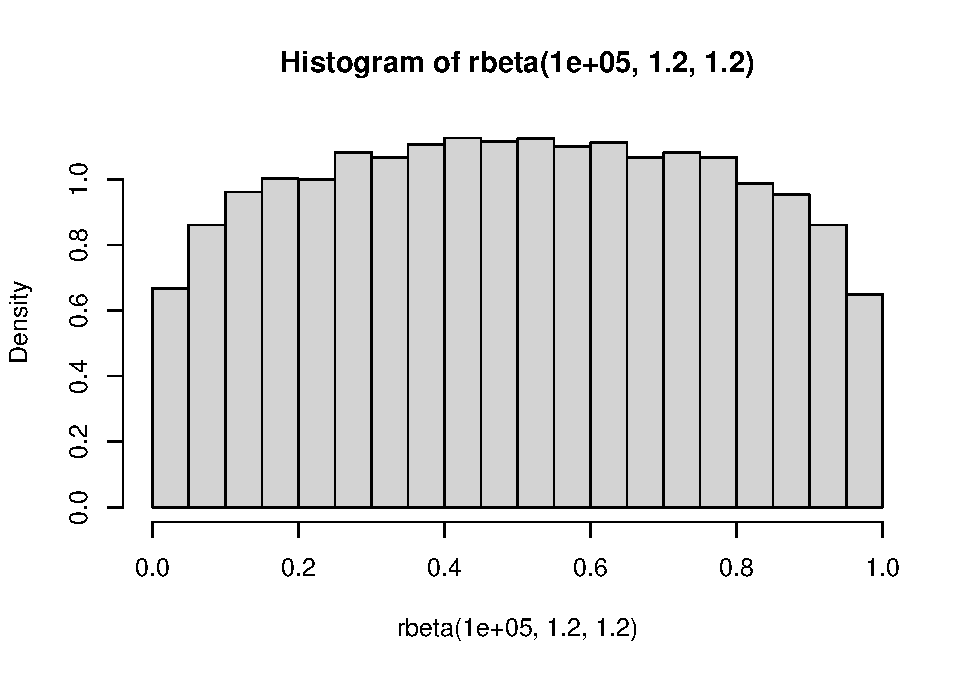
\includegraphics{SAMs_files/figure-latex/unnamed-chunk-22-1.pdf}

This prior is therefore relatively flat and uninformative over the range of plausible values, but provides very weak regularization by giving lower relative probability at the extreme ends approaching 0 (no genetic effect) and 1 (complete genetic effect). With more than two individual-level random effects, such as when specifying multiple matrices of individual autocorrelation \citep{Thomson2018}, SDs and variances can instead be parameterized as scaled \href{https://mc-stan.org/docs/2_19/reference-manual/vector-and-matrix-data-types.html}{simplexes}.

\hypertarget{sam-coding-tutorial}{%
\chapter{SAM coding tutorial}\label{sam-coding-tutorial}}

This section is a work in progress \ldots{}

\hypertarget{coding-the-model}{%
\section{Coding the model}\label{coding-the-model}}

\ldots{}

\hypertarget{quantifying-assortment}{%
\section{Quantifying assortment}\label{quantifying-assortment}}

\ldots{}

\hypertarget{selection-differentials}{%
\section{Selection differentials}\label{selection-differentials}}

\ldots{}

\hypertarget{the-response-to-selection}{%
\section{The response to selection}\label{the-response-to-selection}}

\ldots{}

\hypertarget{extending-sams}{%
\chapter{Extending SAMs}\label{extending-sams}}

This section is a work in progress. Future topics to cover include, among others, SAMs with non-Gaussian phenotypes and fitness measures, social effects due to groups larger than dyads, integrated trait- and variance-partitioning models, and hierarchical phenotypes and latent variable models.

  \bibliography{packages.bib,references.bib}

\end{document}
